	\chapter{Web testing}
	\label{ch:Webtesting}

		There are several approaches for Web testing, the choice among them depends on
		different factors such as lifecycle of the project, technologies used, the
		budget, the professional level of developers. Two main ideas are Capture and
		Replay tests (C\&R) and programmable tests.
		
		\section{Capture and Replay}
		\label{sec:captureReplay}
			C\&R tools have been developed for testing the applications against graphical user interfaces. 
			The software tester works with the Web application modeling user behaviour,
			the C\&R tool records the whole session and generates the
			script, which can be executed later,	repeating same actions without humans participation.
			  The main idea of C\&R
			testing tools is to record a sequence of user actions, that can be
			automatically replayed later and save them in a human readable format. Human
			readable format is an important feature, because script editing might
			 be useful to adjust failed scripts accordingly	to the changes of the Web page.
			 Though if the Web page was changed	significantly, editing test script might be more expensive than recording a
			new test\cite{CaptureReplay7}. 
			
C\&R tools are usually Web browser plugins or Java applets, because they
need to control a Web browser to navigate on a Web page. User actions are
usually saved as a sequence of steps in HTML or XML, which is later used to
generate a Javascript to reproduce user actions. An example of C\&R testing
tool is Selenium IDE described in chapter\ref{ch:selenium}.

The main advantage of C\&R, is that the tester does not
require to have experience in coding. Building test cases with such tools
is a simple task.
The biggest downside of C\&R tests is that editing generated
scripts is harder than editing scripts written by a software
developer\cite{CaptureReplay7}. The test cases are strongly coupled with Web pages and contain hard-coded values. These factors lead to the
problem, that very often the tester have to record a new test, instead of
changing the existing ones.

 When using C\&R tools the tester can
not use loose-coupling, decomposition or other design techniques to make
easy readable and maintainable tests. It is also hard to use parts of already
made test cases when creating new ones. Programmable tests can help to solve these problems.

\section{Programmable tests} 
\label{sec:programTests}
Programmable tests are created by a tester manually. This method requires the
person to have programming skills and takes more time, but programmable tests
are more flexible and allow the developer to use bigger set of tools. The
developer may use conditional statements to change execution of the test,
loops to repeat same actions, exception handling, data structures like
arrays, sets, trees, graphs, logging and etc. Programmable tests are more
flexible and powerful than C\&R tests and provide an opportunity to create
parameterized tests - tests which can be executed multiple times with different arguments. 

Thought writing programmable tests is harder than C\&R and requires more
 experience and skills, programmable tests provide more flexibility and scalability. The empirical study
       of developing tests for four different frameworks shows that the development of programmable tests is more time
      consuming (between 32\% and 112\%), but test maintenance requires less
      time (with a saving of 16\% and 51\%). As a result ``In general, programmable test cases are more
      expensive to write but easier to evolve than C\&R ones, with an advantage
      after two releases (in the median case)''.\cite{CaptureReplay7}

 \section{Capture and Replay vs Programmable tests}
 To show that programmable tests are more powerful than C\&R we provide an
artificial example of testing Vaadin framework.	
Vaadin has a set of UI element classes and we want to	test that changing 
the value of the elements triggers a value change listener event.
First, we create a Web page where we add elements we
want to test such as text field, combo box, radio button. Second, we add a value
change listener to all this elements that will change the value of a test field.
So, when the radio button state changes, event listener method
will change the value of the test field to ``radio button event triggered''. In the test we
iterate through all the elements, change their values and check the value
of the test field see example of test UI \ref{lst:vaadintest} and test case
classes \ref{lst:vaadintest2} in the Appendix A.

The biggest advantage of programmable tests against C\&R is scalability and
better maintainability. When using C\&R a tester should record same actions for
each new element, while with  programmable tests, testing new elements requires
small changes to an existing test case. 

\section {Challenges}
	\label {sec:challenges}
	\subsection{Look and feel testing}
	    Both C\&R and programmable tests are focused on a DOM of the Web page.
	    One disadvantage is they do not provide tools to test appearance of the Web
	    page like colors, margins, fonts, etc. The client side page may have bugs in CSS
	    or HTML, for example if all HTML elements had CSS rule display:none, they
	    would not be shown for a user in the Web browser. Thought all user actions
	    could be still emulated by a testing tool. This problem can be solved by adding screenshot
      comparison see \ref{sec:screencompare}, when a screenshot of a tested Web
      page is compared with a reference screenshot. 
	\subsection{Complex DOM structure}
    Real-life example may have dozens/hundreds of HTML
		elements on the Web page see figure
		\ref{fig:gmailexample}.
		Web pages with big and branched DOM bring several challenges:
		\begin{enumerate}
		  \item Searching for required element may be very resource-consuming,
		  affecting time of the test execution. 
		  \item Changes in DOM may require changes in tests, which increase
		  application maintenance costs.
		\end{enumerate}
		
		\begin{figure}
		\centering
		  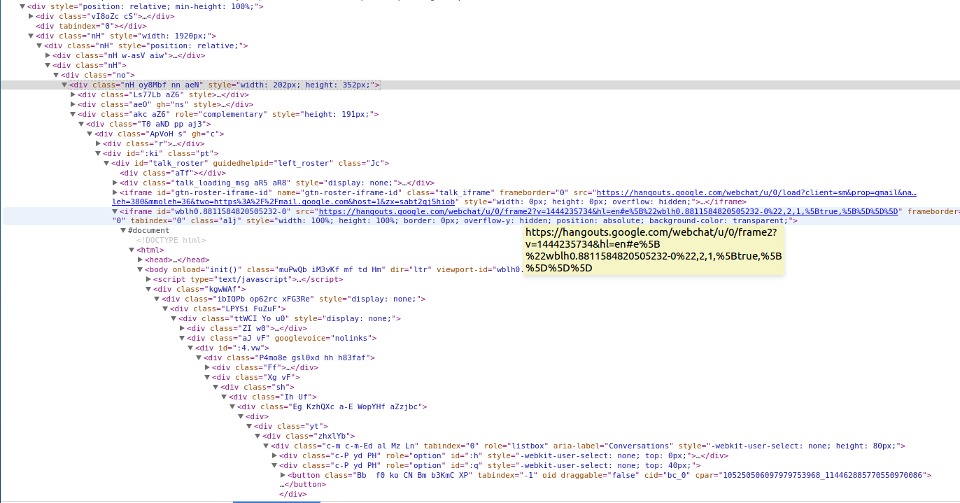
\includegraphics[width=0.75\textwidth]{gmail_example}
		  \caption{Gmail page structure}
		  \label{fig:gmailexample}
		\end{figure}
		
		Testing frameworks allow several strategies for locating Web page elements:
		\begin{enumerate}
		  \item By id - locates the Web page elements using their id values.
		  \item By name - locates the Web page elements using their name.
		  \item By tag - locates the Web page elements using their tag.
		  \item By class - locates the Web page elements using their class attribute.
		  \item By XPath - combines previous strategies and builds a search
		  path to an element in the DOM.
		\end{enumerate}
		
		The efficiency between these strategies is a trade-off between effeciency of
		the test and its complexity for developer. An industrial case study shows that 
		XPath methods for locating elements on a Web page take 
		three times longer than same tests with searching
    elements by id\cite{selenium4}. 
	   Id-based tests for static HTML Web pages with small amount of elements
	   is an optimal solution. On the contarary, in case of dynamically
	   generated HTML with many elements as in example \ref{fig:gmailexample}
	   searching elements by id is inappropriate.
		
		The biggest downside of searching by id strategy, is that every HTML element
		should have a unique ID. If the Web pages has a dynamically generated content,
		for example a table, where amount of rows depends on data, the
		developer has to add some logic to generate ID for each row and also verify
		that new ids do not conflict with already created ones. 
		
		In some circumstances the developer needs to get a set of elements by some
		criteria, for example get all elements with a specific tag or class selector
		and process them in a loop. 
		
		As we can see there is no one solution for searching elements on a Web page,
		which can be used in all cases. The developer should make a solution which
		searching algorithm to use based on requirements, but the testing framework
		should provide the developer different tools to choose from. In chapter
		\ref{ch:selenium} we will present Selenium - a software testing framework
		for Web applications, which allows to create C\&R \ref{sec:captureReplay} and 
    programmable tests \ref{sec:programTests}. Selenium  supports searching
    elements by id,tag, class, XPath, etc and provides an opportunity simulate
    user actions on a Web page.
		

 